\documentclass[11pt,a4paper]{report}
\usepackage[textwidth=37em,vmargin=30mm]{geometry}
\usepackage{calc,xunicode,amsmath,amssymb,paralist,enumitem,tabu,booktabs,datetime2,xeCJK,xeCJKfntef,listings}
\usepackage{tocloft,fancyhdr,tcolorbox,xcolor,graphicx,eso-pic,xltxtra,xelatexemoji}

\newcommand{\envyear}[0]{2025}
\newcommand{\envdatestr}[0]{2025-06-09}
\newcommand{\envfinaldir}[0]{webdb/2025/20250609/final}

\usepackage[hidelinks]{hyperref}
\hypersetup{
    colorlinks=false,
    pdfpagemode=FullScreen,
    pdftitle={Web Digest - \envdatestr}
}

\setlength{\cftbeforechapskip}{10pt}
\renewcommand{\cftchapfont}{\rmfamily\bfseries\large\raggedright}
\setlength{\cftbeforesecskip}{2pt}
\renewcommand{\cftsecfont}{\sffamily\small\raggedright}

\setdefaultleftmargin{2em}{2em}{1em}{1em}{1em}{1em}

\usepackage{xeCJK,xeCJKfntef}
\xeCJKsetup{PunctStyle=plain,RubberPunctSkip=false,CJKglue=\strut\hskip 0pt plus 0.1em minus 0.05em,CJKecglue=\strut\hskip 0.22em plus 0.2em}
\XeTeXlinebreaklocale "zh"
\XeTeXlinebreakskip = 0pt


\setmainfont{Brygada 1918}
\setromanfont{Brygada 1918}
\setsansfont{IBM Plex Sans}
\setmonofont{JetBrains Mono NL}
\setCJKmainfont{Noto Serif CJK SC}
\setCJKromanfont{Noto Serif CJK SC}
\setCJKsansfont{Noto Sans CJK SC}
\setCJKmonofont{Noto Sans CJK SC}

\setlength{\parindent}{0pt}
\setlength{\parskip}{8pt}
\linespread{1.15}

\lstset{
	basicstyle=\ttfamily\footnotesize,
	numbersep=5pt,
	backgroundcolor=\color{black!5},
	showspaces=false,
	showstringspaces=false,
	showtabs=false,
	tabsize=2,
	captionpos=b,
	breaklines=true,
	breakatwhitespace=true,
	breakautoindent=true,
	linewidth=\textwidth
}






\newcommand{\coverpic}[2]{
    % argv: itemurl, authorname
    Cover photo by #2~~(\href{#1}{#1})
}
\newcommand{\makeheader}[0]{
    \begin{titlepage}
        % \newgeometry{hmargin=15mm,tmargin=21mm,bmargin=12mm}
        \begin{center}
            
            \rmfamily\scshape
            \fontspec{BaskervilleF}
            \fontspec{Old Standard}
            \fontsize{59pt}{70pt}\selectfont
            WEB\hfill DIGEST
            
            \vfill
            % \vskip 30pt
            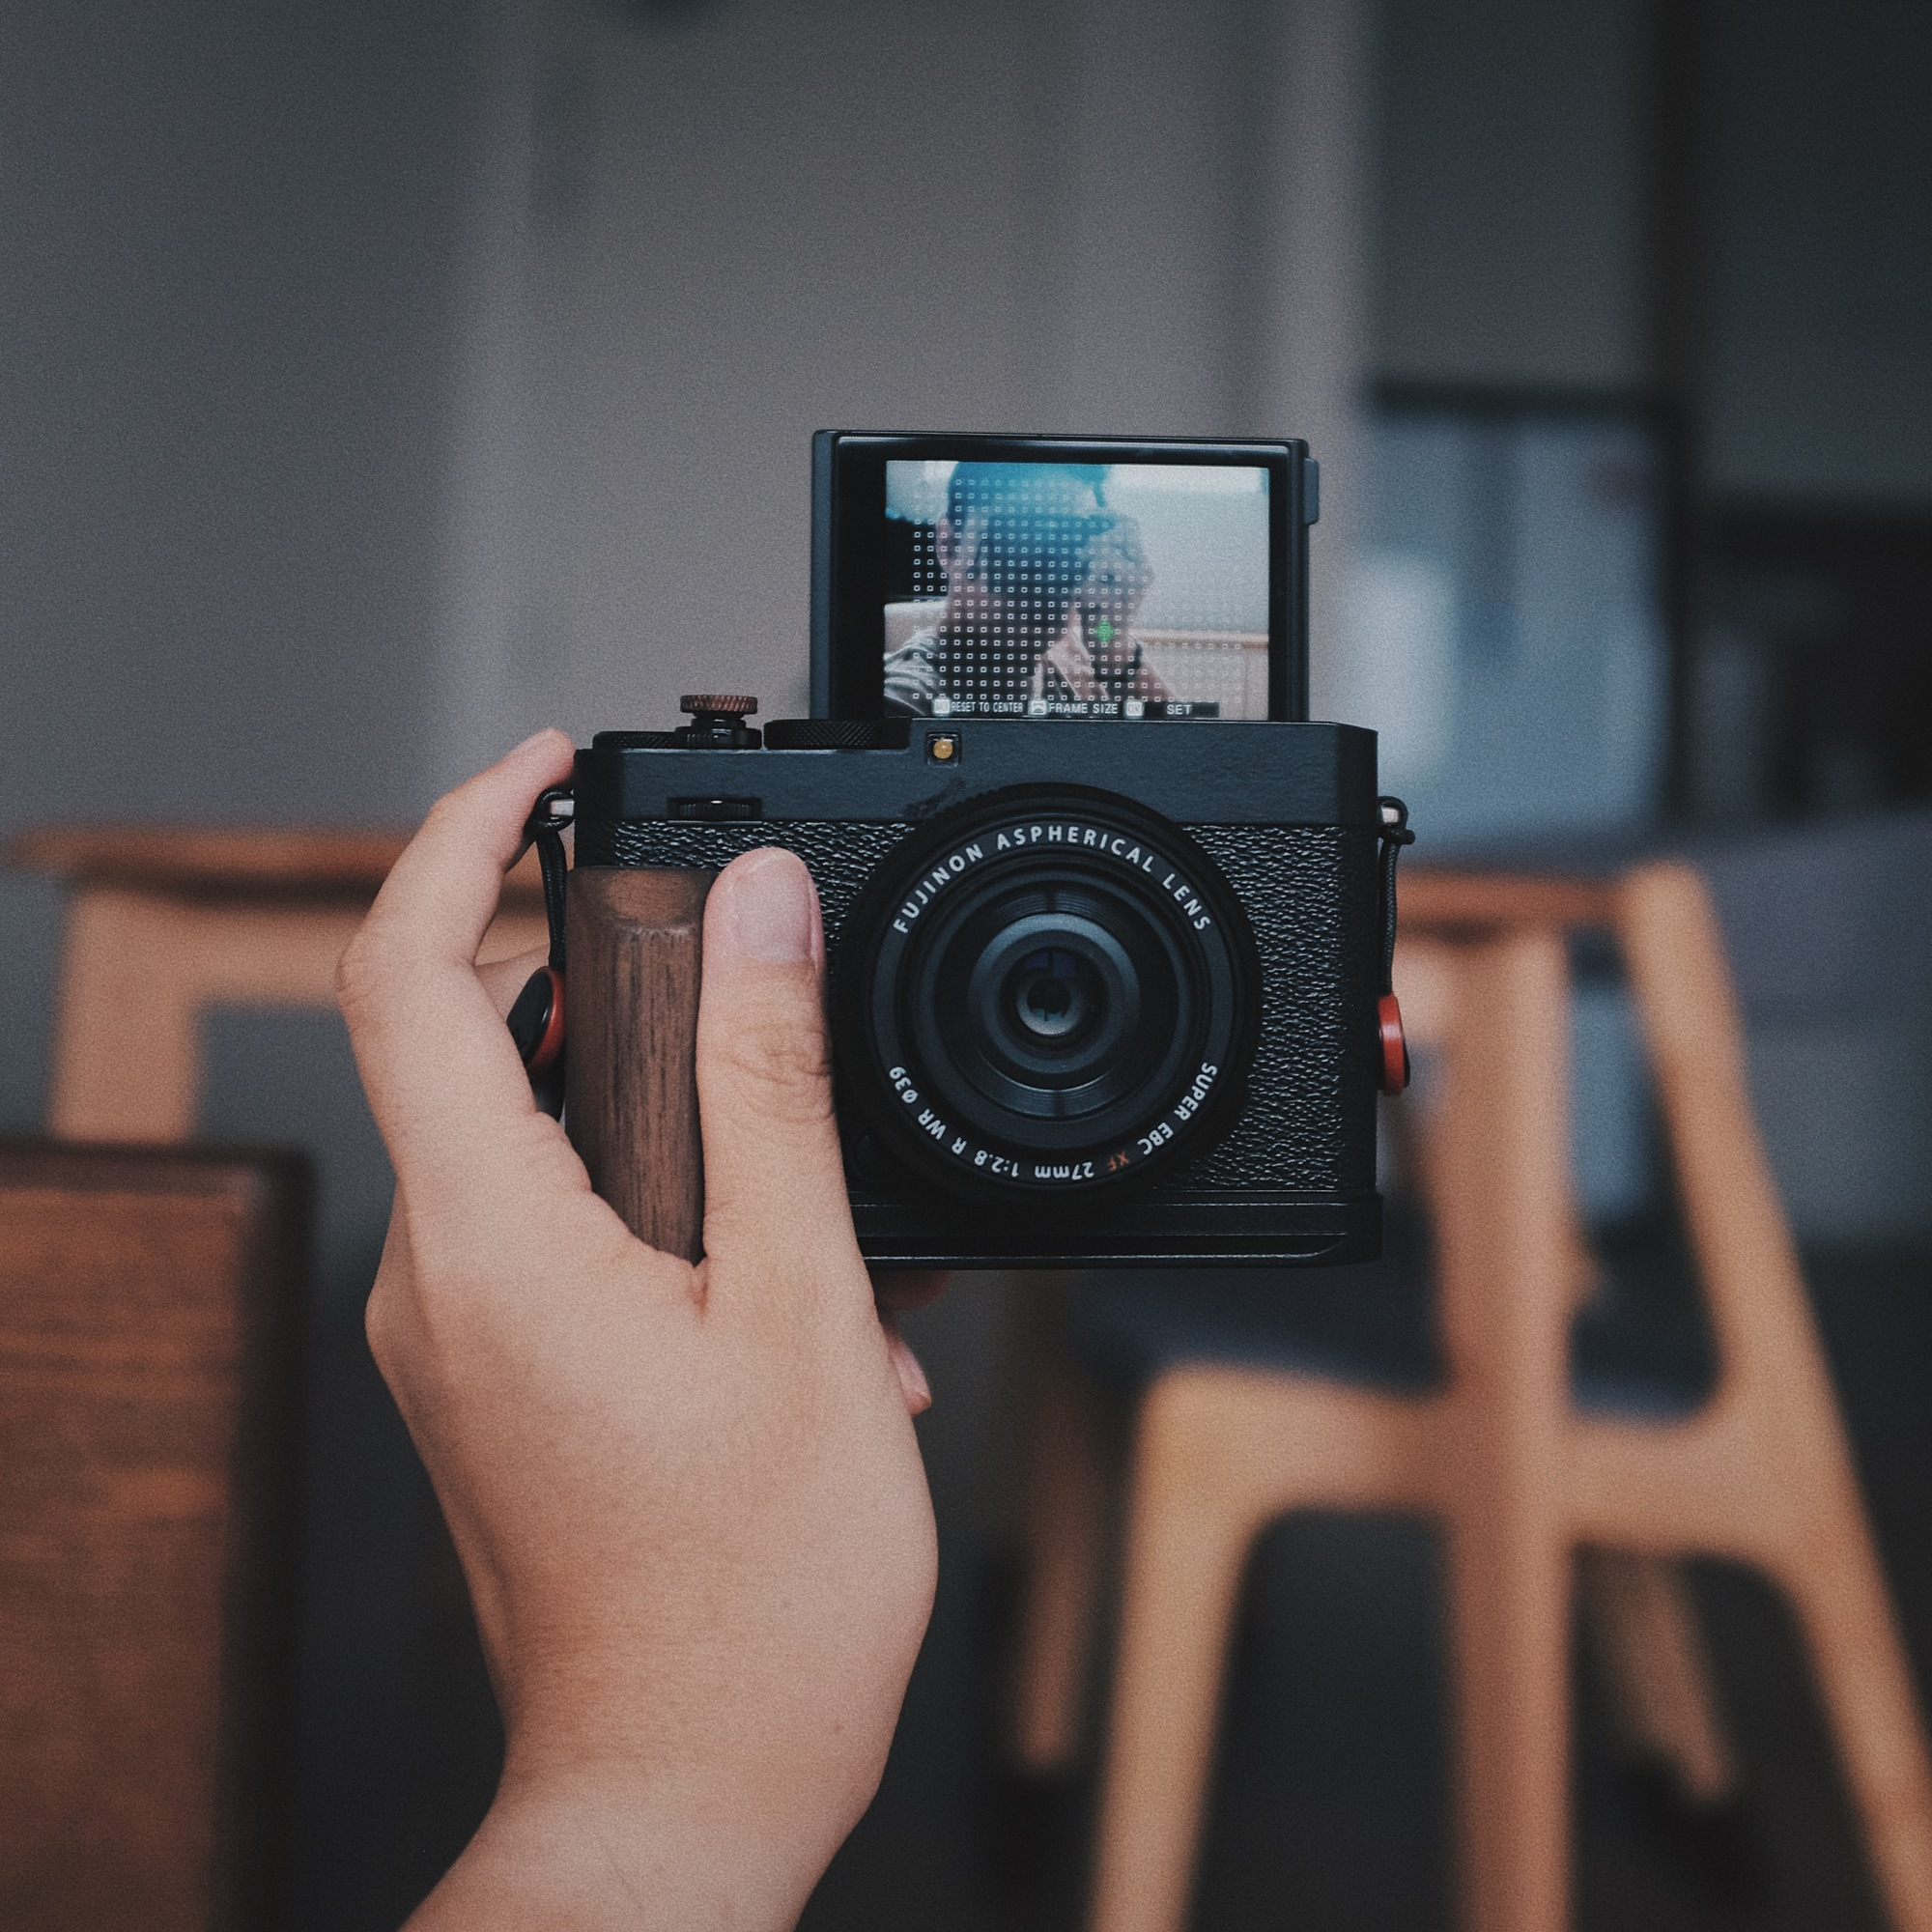
\includegraphics[width=\linewidth]{\envfinaldir/coverpic-prod.jpg}\par
            % \vskip 30pt
            \vfill

            \normalsize\rmfamily\scshape
            \copyright{} The Web Digest Project \hfill\large \envdatestr
        \end{center}
    \end{titlepage}
    % \restoregeometry
}
\newcommand{\simplehref}[1]{%
    \textcolor{blue!80!green}{\href{#1}{#1}}%
}
\renewcommand{\contentsname}{\center\Huge\sffamily\bfseries Contents\par\vskip 20pt}
\newcounter{ipartcounter}
\setcounter{ipartcounter}{0}
\newcommand{\ipart}[1]{
    % \vskip 20pt
    \clearpage
    \stepcounter{ipartcounter}
    \phantomsection
    \addcontentsline{toc}{chapter}{#1}
    % \begin{center}
    %     \Huge
    %     \sffamily\bfseries
    %     #1
    % \end{center}
    % \vskip 20pt plus 7pt
}
\newcounter{ichaptercounter}
\setcounter{ichaptercounter}{0}
\newcommand{\ichapter}[1]{
    % \vskip 20pt
    \clearpage
    \stepcounter{ichaptercounter}
    \phantomsection
    \addcontentsline{toc}{section}{\numberline{\arabic{ichaptercounter}}#1}
    \begin{center}
        \Huge
        \sffamily\bfseries
        #1
    \end{center}
    \vskip 20pt plus 7pt
}
\newcommand{\entrytitlefont}[1]{\subsection*{\raggedright\Large\sffamily\bfseries#1}}
\newcommand{\entryitemGeneric}[2]{
    % argv: title, url
    \parbox{\linewidth}{
        \entrytitlefont{#1}\par\vskip 5pt
        \footnotesize\ttfamily\mdseries
        \simplehref{#2}
    }\vskip 11pt plus 11pt minus 1pt
}
\newcommand{\entryitemGithub}[3]{
    % argv: title, url, desc
    \parbox{\linewidth}{
        \entrytitlefont{#1}\par\vskip 5pt
        \footnotesize\ttfamily\mdseries
        \simplehref{#2}\par\vskip 5pt
        \small\rmfamily\mdseries#3
    }\vskip 11pt plus 11pt minus 1pt
}
\newcommand{\entryitemAp}[3]{
    % argv: title, url, desc
    \parbox{\linewidth}{
        \entrytitlefont{#1}\par\vskip 5pt
        \footnotesize\ttfamily\mdseries
        \simplehref{#2}\par\vskip 5pt
        \small\rmfamily\mdseries#3
    }\vskip 11pt plus 11pt minus 1pt
}
\newcommand{\entryitemHackernews}[3]{
    % argv: title, hnurl, rawurl
    % \parbox{\linewidth}{
    %     \entrytitlefont{#1}\par\vskip 5pt
    %     \footnotesize\ttfamily\mdseries
    %     \simplehref{#3}\par
    %     \textcolor{black!50}{\href{#2}{#2}}
    % }\vskip 11pt plus 11pt minus 1pt
    \begin{minipage}{\linewidth}
            \entrytitlefont{#1}\par\vskip 5pt
            \footnotesize\ttfamily\mdseries
            \simplehref{#3}\par
            \textcolor{black!50}{\href{#2}{#2}}
    \end{minipage}\par\vskip 11pt plus 11pt minus 1pt
}







\begin{document}

\makeheader

\tableofcontents\clearpage




\ipart{Developers}
\ichapter{Hacker News}
\entryitemTwoLinks{Why Android can't use CDC Ethernet (2023)}{https://news.ycombinator.com/item?id=44219405}{https://jordemort.dev/blog/why-android-cant-use-cdc-ethernet/}

\entryitemTwoLinks{Administering immunotherapy in the morning seems to matter. Why?}{https://news.ycombinator.com/item?id=44217876}{https://www.owlposting.com/p/the-time-of-day-that-immunotherapy}

\entryitemTwoLinks{Ask HN: How to learn CUDA to professional level}{https://news.ycombinator.com/item?id=44216123}{https://news.ycombinator.com/item?id=44216123}

\entryitemTwoLinks{A look at Cloudflare's AI-coded OAuth library}{https://news.ycombinator.com/item?id=44215667}{https://neilmadden.blog/2025/06/06/a-look-at-cloudflares-ai-coded-oauth-library/}

\entryitemTwoLinks{Why not use DNS over HTTPS (DoH)?}{https://news.ycombinator.com/item?id=44215608}{https://www.bsdhowto.ch/doh.html}

\entryitemTwoLinks{Gaussian integration is cool}{https://news.ycombinator.com/item?id=44215603}{https://rohangautam.github.io/blog/chebyshev\_gauss/}

\entryitemTwoLinks{The last six months in LLMs, illustrated by pelicans on bicycles}{https://news.ycombinator.com/item?id=44215352}{https://simonwillison.net/2025/Jun/6/six-months-in-llms/}

\entryitemTwoLinks{The Illusion of Thinking: Strengths and Limitations of Reasoning Models}{https://news.ycombinator.com/item?id=44215273}{https://machinelearning.apple.com/research/illusion-of-thinking}

\entryitemTwoLinks{Reverse engineering Claude Code}{https://news.ycombinator.com/item?id=44214926}{https://kirshatrov.com/posts/claude-code-internals}

\entryitemTwoLinks{Maintaining an Android app in Google Play Store is a lot of work}{https://news.ycombinator.com/item?id=44214835}{https://ashishb.net/programming/maintaining-android-app/}

\entryitemTwoLinks{<Blink> and <Marquee> (2020)}{https://news.ycombinator.com/item?id=44214522}{https://danq.me/2020/11/11/blink-and-marquee/}

\entryitemTwoLinks{Knowledge Management in the Age of AI}{https://news.ycombinator.com/item?id=44214481}{https://ericgardner.info/notes/knowledge-management-june-2025}

\entryitemTwoLinks{Louis Rossmann: We've started a foundation to bring back ownership [video]}{https://news.ycombinator.com/item?id=44214311}{https://www.youtube.com/watch?v=WBG6Vw3nxZs}

\entryitemTwoLinks{You need much less memory than time}{https://news.ycombinator.com/item?id=44212855}{https://blog.computationalcomplexity.org/2025/02/you-need-much-less-memory-than-time.html}

\entryitemTwoLinks{Coventry Very Light Rail}{https://news.ycombinator.com/item?id=44212845}{https://www.coventry.gov.uk/coventry-light-rail}

\entryitemTwoLinks{Convert photos to Atkinson dithering}{https://news.ycombinator.com/item?id=44212446}{https://gazs.github.io/canvas-atkinson-dither/}

\entryitemTwoLinks{Joining Apple Computer (2018)}{https://news.ycombinator.com/item?id=44212441}{https://www.folklore.org/Joining\_Apple\_Computer.html}

\entryitemTwoLinks{Discovering a JDK Race Condition, and Debugging It in 30 Minutes with Fray}{https://news.ycombinator.com/item?id=44211779}{https://aoli.al/blogs/jdk-bug/}

\entryitemTwoLinks{BorgBackup 2 has no server-side append-only anymore}{https://news.ycombinator.com/item?id=44211612}{https://github.com/borgbackup/borg/pull/8798}

\entryitemTwoLinks{Field Notes from Shipping Real Code with Claude}{https://news.ycombinator.com/item?id=44211417}{https://diwank.space/field-notes-from-shipping-real-code-with-claude}\ichapter{GitHub}
\entryitemWithDescription{\hskip 0pt{}codecrafters-io/build-your-own-x}{https://github.com/codecrafters-io/build-your-own-x}{Master programming by recreating your favorite technologies from
scratch.\\
Language: Markdown\\
Stars: 385644\\
Forks: 35968}\ichapter{Dribbble}
\entryitemGeneric{\hskip 0pt{}Aquasan}{https://dribbble.com/shots/26100535-Aquasan}

\entryitemGeneric{\hskip 0pt{}Eagle}{https://dribbble.com/shots/26099428-Eagle}

\entryitemGeneric{\hskip 0pt{}Mnp Technologies - Logo Design}{https://dribbble.com/shots/26092034-Mnp-Technologies-Logo-Design}

\entryitemGeneric{\hskip 0pt{}Singular Logo Concept (Unused)}{https://dribbble.com/shots/26091755-Singular-Logo-Concept-Unused}

\entryitemGeneric{\hskip 0pt{}Cre8tera // Website}{https://dribbble.com/shots/26091009-Cre8tera-Website}

\entryitemGeneric{\hskip 0pt{}Cool Pool Logo Design - Letter C Monogram}{https://dribbble.com/shots/26091401-Cool-Pool-Logo-Design-Letter-C-Monogram}

\entryitemGeneric{\hskip 0pt{}Gorilla + Bar Chart Logo}{https://dribbble.com/shots/26092670-Gorilla-Bar-Chart-Logo}

\entryitemGeneric{\hskip 0pt{}zeero logo design}{https://dribbble.com/shots/26087342-zeero-logo-design}

\entryitemGeneric{\hskip 0pt{}Create email inbox composition}{https://dribbble.com/shots/26083118-Create-email-inbox-composition}

\entryitemGeneric{\hskip 0pt{}Shori Brand}{https://dribbble.com/shots/26088139-Shori-Brand}

\entryitemGeneric{\hskip 0pt{}Roaring Bear}{https://dribbble.com/shots/26087788-Roaring-Bear}

\entryitemGeneric{\hskip 0pt{}Eagle}{https://dribbble.com/shots/26085536-Eagle}

\entryitemGeneric{\hskip 0pt{}Hand-drawn illustration pack}{https://dribbble.com/shots/26084735-Hand-drawn-illustration-pack}

\entryitemGeneric{\hskip 0pt{}Dog Mascot Various Poses}{https://dribbble.com/shots/26087977-Dog-Mascot-Various-Poses}

\entryitemGeneric{\hskip 0pt{}Branding Concept for Europe}{https://dribbble.com/shots/26087652-Branding-Concept-for-Europe}

\entryitemGeneric{\hskip 0pt{}B2B Dashboard \& Web App UI UX Design for Carbon Solutions}{https://dribbble.com/shots/26076624-B2B-Dashboard-Web-App-UI-UX-Design-for-Carbon-Solutions}

\entryitemGeneric{\hskip 0pt{}Patriot Logo Design (Unused for Sale)}{https://dribbble.com/shots/26081047-Patriot-Logo-Design-Unused-for-Sale}

\entryitemGeneric{\hskip 0pt{}Heliopoint}{https://dribbble.com/shots/26081987-Heliopoint}

\entryitemGeneric{\hskip 0pt{}Apple}{https://dribbble.com/shots/26084067-Apple}

\entryitemGeneric{\hskip 0pt{}Illustration}{https://dribbble.com/shots/26083223-Illustration}

\entryitemGeneric{\hskip 0pt{}Europe Logo Animation}{https://dribbble.com/shots/26082596-Europe-Logo-Animation}

\entryitemGeneric{\hskip 0pt{}Arc Logo}{https://dribbble.com/shots/26083648-Arc-Logo}

\entryitemGeneric{\hskip 0pt{}Heyo Turns 2!}{https://dribbble.com/shots/26078572-Heyo-Turns-2}

\entryitemGeneric{\hskip 0pt{}Fox Brand Mascot}{https://dribbble.com/shots/26077954-Fox-Brand-Mascot}


\ipart{Developers~~~~(zh-Hans)}
\ichapter{Solidot}
\entryitemGeneric{\hskip 0pt{}/e/OS 3.0 释出}{https://www.solidot.org/story?sid=81498}

\entryitemGeneric{\hskip 0pt{}Android 应用面临越来越多的不兼容问题}{https://www.solidot.org/story?sid=81497}

\entryitemGeneric{\hskip 0pt{}越南废除二孩政策}{https://www.solidot.org/story?sid=81496}

\entryitemGeneric{\hskip 0pt{}天文学家发现中等质量黑洞的新证据}{https://www.solidot.org/story?sid=81495}

\entryitemGeneric{\hskip 0pt{}英国考虑推出数字 ID 卡}{https://www.solidot.org/story?sid=81494}

\entryitemGeneric{\hskip 0pt{}就读美国大学的中国留学生人数持续下降}{https://www.solidot.org/story?sid=81493}

\entryitemGeneric{\hskip 0pt{}YouTube 以有害内容下架主播的自我托管视频内容的教程}{https://www.solidot.org/story?sid=81492}

\entryitemGeneric{\hskip 0pt{}德国数字部长呼吁在开放标准和开源的原则下开发欧洲 IT 解决方案}{https://www.solidot.org/story?sid=81490}

\entryitemGeneric{\hskip 0pt{}阿里云遭遇域名解析故障}{https://www.solidot.org/story?sid=81489}

\entryitemGeneric{\hskip 0pt{}科学家通过脑机接口恢复失明动物视觉功能}{https://www.solidot.org/story?sid=81488}

\entryitemGeneric{\hskip 0pt{}日 ispace 登月尝试再次失败}{https://www.solidot.org/story?sid=81487}

\entryitemGeneric{\hskip 0pt{}加州法庭裁决驾驶时在手机上查地图违法}{https://www.solidot.org/story?sid=81486}

\entryitemGeneric{\hskip 0pt{}海南政府试点跨境加速服务}{https://www.solidot.org/story?sid=81485}

\entryitemGeneric{\hskip 0pt{}在传出 OpenAI 准备收购 Windsurf 后 Anthropic 切断了该公司对其大模型的访问}{https://www.solidot.org/story?sid=81484}

\entryitemGeneric{\hskip 0pt{}亚马逊测试用人形机器人送包裹}{https://www.solidot.org/story?sid=81483}

\entryitemGeneric{\hskip 0pt{}美洲原住民在千年前就以集约化方式种植玉米}{https://www.solidot.org/story?sid=81482}\ichapter{V2EX}
\entryitemGeneric{\hskip 0pt{}[汽车] 二手车选购建议: Model3 还是森林人}{https://www.v2ex.com/t/1137252}

\entryitemGeneric{\hskip 0pt{}[反馈] 鸿蒙 NEXT 手机访问 V2EX 显示的是 PC 端界面}{https://www.v2ex.com/t/1137251}

\entryitemGeneric{\hskip 0pt{}[macOS] Mac - 订阅 Up 主最新动态的 推送聚合软件(B 站,油管, Reddit,抖音 等)}{https://www.v2ex.com/t/1137250}

\entryitemGeneric{\hskip 0pt{}[生活] 分享一次我用 Google gemini 维修家电的经历}{https://www.v2ex.com/t/1137249}

\entryitemGeneric{\hskip 0pt{}[掌机] 微软和华硕联合打造的 Xbox 掌机正式官宣了}{https://www.v2ex.com/t/1137247}

\entryitemGeneric{\hskip 0pt{}[NAS] tailscale subnet 的问题}{https://www.v2ex.com/t/1137246}

\entryitemGeneric{\hskip 0pt{}[NAS] 绿联 DXP4800 这台可以刷飞牛 OS 么}{https://www.v2ex.com/t/1137245}

\entryitemGeneric{\hskip 0pt{}[程序员] 万能的 V 友,推荐点类似 FastGPT 的项目}{https://www.v2ex.com/t/1137244}

\entryitemGeneric{\hskip 0pt{}[OpenWrt] 请问大佬, iStore os 做主路由后端口转发的问题}{https://www.v2ex.com/t/1137243}

\entryitemGeneric{\hskip 0pt{}[分享发现] perplexity 年度会员}{https://www.v2ex.com/t/1137242}

\entryitemGeneric{\hskip 0pt{}[问与答] 现在国补都不能延迟发货了?}{https://www.v2ex.com/t/1137241}

\entryitemGeneric{\hskip 0pt{}[分享创造] LLM Background Diagnostics vscode Extension}{https://www.v2ex.com/t/1137240}

\entryitemGeneric{\hskip 0pt{}[程序员] 谷歌走了这么多年了, 国内就没人想打败百度?}{https://www.v2ex.com/t/1137239}

\entryitemGeneric{\hskip 0pt{}[酷工作] 字节阿里大公司梦}{https://www.v2ex.com/t/1137236}

\entryitemGeneric{\hskip 0pt{}[分享创造] 极简图片风格转换,专注解决三大核心痛点}{https://www.v2ex.com/t/1137235}

\entryitemGeneric{\hskip 0pt{}[Linux] windows APP 连接远程 ubuntu}{https://www.v2ex.com/t/1137233}

\entryitemGeneric{\hskip 0pt{}[问与答] 2025 年 6 月,求推荐款显示器}{https://www.v2ex.com/t/1137232}

\entryitemGeneric{\hskip 0pt{}[Apple] Perplexity 领取一年免费会员}{https://www.v2ex.com/t/1137230}

\entryitemGeneric{\hskip 0pt{}[程序员] CAN 总线通信不稳定的问题}{https://www.v2ex.com/t/1137229}

\entryitemGeneric{\hskip 0pt{}[北京] 问下大家是怎么租到便宜又合适的房子的}{https://www.v2ex.com/t/1137227}

\entryitemGeneric{\hskip 0pt{}[问与答] 招商银行 ATM 为什么现在已经不支持手机 Pay 取款, 也取消了扫码存款}{https://www.v2ex.com/t/1137226}

\entryitemGeneric{\hskip 0pt{}[问与答] 安桥 RZ50 AVR 搭配一个双声道后级功放推主箱}{https://www.v2ex.com/t/1137224}

\entryitemGeneric{\hskip 0pt{}[分享创造] 我开发了一个图片混淆工具}{https://www.v2ex.com/t/1137223}

\entryitemGeneric{\hskip 0pt{}[NAS] 群晖 nas 温度超过 90 度关机}{https://www.v2ex.com/t/1137221}

\entryitemGeneric{\hskip 0pt{}[分享发现] intel 显卡跑 Qwen3-14B-GGUF:Q8\_0}{https://www.v2ex.com/t/1137219}

\entryitemGeneric{\hskip 0pt{}[分享发现] 你们的 edge 浏览器是这样吗,一堆负优化}{https://www.v2ex.com/t/1137218}

\entryitemGeneric{\hskip 0pt{}[分享发现] 某搜索引擎给出错误的无铅焊锡温度}{https://www.v2ex.com/t/1137217}

\entryitemGeneric{\hskip 0pt{}[小米] 有没有适合夏天用的小米手环腕带}{https://www.v2ex.com/t/1137215}

\entryitemGeneric{\hskip 0pt{}[生活] 小孩轻度近视,医生说近距离看书写字也要一直佩戴眼镜,不大理解?}{https://www.v2ex.com/t/1137212}

\entryitemGeneric{\hskip 0pt{}[汽车] 买车求推荐,预算在落地价 10W-14W。}{https://www.v2ex.com/t/1137211}

\entryitemGeneric{\hskip 0pt{}[问与答] 求 v 友推荐一款父母用的手机,准备在小黄鱼淘一个,二手价格的预算在 1k—2k,在意续航和耐造,其他的能用就行}{https://www.v2ex.com/t/1137208}

\entryitemGeneric{\hskip 0pt{}[路由器] 手机 wifi 漫游,会导致 ros 地址池被占满}{https://www.v2ex.com/t/1137207}

\entryitemGeneric{\hskip 0pt{}[问与答] 有没有迷你主机推荐一下? 主要是办公和玩普通网游, 像原神/英雄联盟这些}{https://www.v2ex.com/t/1137206}

\entryitemGeneric{\hskip 0pt{}[投资] 你们的投资策略是什么}{https://www.v2ex.com/t/1137205}

\entryitemGeneric{\hskip 0pt{}[分享创造] js-syntax.com 检测 JS 语法特性的网站}{https://www.v2ex.com/t/1137204}

\entryitemGeneric{\hskip 0pt{}[Android] 请问酷比魔方 iplay50pro 是原生系统好,还是刷成 miui 好?}{https://www.v2ex.com/t/1137203}

\entryitemGeneric{\hskip 0pt{}[分享发现] kimi 这😂}{https://www.v2ex.com/t/1137201}

\entryitemGeneric{\hskip 0pt{}[Tesla] 还是很纠结长续和标续}{https://www.v2ex.com/t/1137199}

\entryitemGeneric{\hskip 0pt{}[问与答] 如何查看京东家电历史到手价格}{https://www.v2ex.com/t/1137198}

\entryitemGeneric{\hskip 0pt{}[React] gpt 给我搞懵了,是我对 Suspense 理解有误吗?}{https://www.v2ex.com/t/1137197}

\entryitemGeneric{\hskip 0pt{}[分享发现] 花了半个下午看看有没有办法从我的划船机导出实时运动数据}{https://www.v2ex.com/t/1137196}

\entryitemGeneric{\hskip 0pt{}[职场话题] 职业方向的艰难选择}{https://www.v2ex.com/t/1137192}

\entryitemGeneric{\hskip 0pt{}[Apple] 求问: Mac 应用 or 系统安装到外置硬盘的经验}{https://www.v2ex.com/t/1137191}

\entryitemGeneric{\hskip 0pt{}[全球工单系统] VVebo 今天彻底挂了?}{https://www.v2ex.com/t/1137189}

\entryitemGeneric{\hskip 0pt{}[问与答] aistudio 的模型 gem 2.5 pro 怎样接到 vscode 或者 cursor,让我可以把 代码上下文 传给它?}{https://www.v2ex.com/t/1137188}

\entryitemGeneric{\hskip 0pt{}[Apple] 1452 的 Dell S2725QS 是不是可以无脑冲了}{https://www.v2ex.com/t/1137187}

\entryitemGeneric{\hskip 0pt{}[Apple] 我只想知道大家是如何屏蔽摇一摇跳转的?}{https://www.v2ex.com/t/1137185}

\entryitemGeneric{\hskip 0pt{}[深圳] 购物公园附近上班,求租房建议}{https://www.v2ex.com/t/1137182}

\entryitemGeneric{\hskip 0pt{}[酷工作] [上海] [宝可梦] AI 开发工程师}{https://www.v2ex.com/t/1137181}

\entryitemGeneric{\hskip 0pt{}[程序员] 腾讯电脑管家 怎么关闭本地文件搜索工具进程?}{https://www.v2ex.com/t/1137180}


\ipart{Generic News}
\ichapter{AP News}
\entryitemWithDescription{\hskip 0pt{}Michaels completes acquisition of Joann's intellectual property and fan-favorite labels}{https://apnews.com/article/c57cae0101fc31da0661c69691066bf5}{}

\entryitemWithDescription{\hskip 0pt{}Midea recalling 1.7 million of its popular air conditioners due to mold concern}{https://apnews.com/article/59e18fb2ecce43711d794c2ca7802ce8}{}

\entryitemWithDescription{\hskip 0pt{}Police consider whether `King of the Hill' actor's sexual orientation played a role in his killing}{https://apnews.com/article/741890b752b0a2a4f8fa8a661bc0c5a1}{}

\entryitemWithDescription{\hskip 0pt{}What to know about the much-anticipated Nintendo Switch 2 on launch day}{https://apnews.com/article/5c8164c9f4dbac998962de29f24947d2}{}

\entryitemWithDescription{\hskip 0pt{}FanDuel bans bettor over heckling incident with Olympic champion sprinter Gabby Thomas}{https://apnews.com/article/d226103292fdf6c019f0c71435e9745e}{}

\entryitemWithDescription{\hskip 0pt{}Ex-White House press secretary Karine Jean-Pierre left Democratic Party, publisher of her book says}{https://apnews.com/article/fbb44b9eb3bb56f6ab8ef02bd7ffa042}{}

\entryitemWithDescription{\hskip 0pt{}Dilly Dally the sea turtle returns to the ocean after flipper amputation}{https://apnews.com/article/3310f37f8901e539453c22ca40dabc00}{}

\entryitemWithDescription{\hskip 0pt{}Hegseth orders the name of gay rights activist Harvey Milk scrubbed from Navy ship}{https://apnews.com/article/d6cda5df15ee5bc066092d54c591c6f2}{}

\entryitemWithDescription{\hskip 0pt{}Reddit sues AI company Anthropic for allegedly `scraping' user comments to train chatbot Claude}{https://apnews.com/article/f5ea042beb253a3f05a091e70531692d}{}

\entryitemWithDescription{\hskip 0pt{}A long-running experiment finds a tiny particle is still acting weird}{https://apnews.com/article/cb123cd20bfd8141dbf75de62804b32b}{}

\entryitemWithDescription{\hskip 0pt{}Woman who denies mushroom murders of her in-laws accepts that she served them death caps for lunch}{https://apnews.com/article/00ea28021943fe4a56d2a3b30ad26598}{}

\entryitemWithDescription{\hskip 0pt{}Northern lights could be visible again in some US states after weekend solar storms}{https://apnews.com/article/915a2364b24679c63a07066f55c53ffa}{}

\entryitemWithDescription{\hskip 0pt{}Eagles' Saquon Barkley announced as Madden NFL 26 cover athlete}{https://apnews.com/article/3b0254fa10fb8df98e91562be76d8d5c}{}\ichapter{Reuters}
\entryitemWithDescription{\hskip 0pt{}Political divide widens as Trump deploys National Guard to Los Angeles}{https://www.reuters.com/world/us/political-divide-widens-trump-deploys-national-guard-los-angeles-2025-06-08/}{The protests against the raids have fueled discussion on the boundaries of presidential power and the public\textquotesingle s right to...}

\entryitemWithDescription{\hskip 0pt{}Ukraine's Zelenskiy vows to press on with prisoner exchanges with Russia}{https://www.reuters.com/world/ukraines-zelenskiy-vows-press-with-prisoner-exchanges-with-russia-2025-06-08/}{Ukrainian President Volodymyr Zelenskiy vowed on Sunday to press on with prisoner exchanges with Russia and said any failure by Moscow to uphold humanitarian accords cast doubt over U.S. and other efforts to end the more than three-year...}

\entryitemWithDescription{\hskip 0pt{}Israel reveals tunnel under Gaza hospital, says body of Sinwar's brother found there}{https://www.reuters.com/world/middle-east/israel-reveals-tunnel-under-gaza-hospital-says-body-sinwars-brother-found-there-2025-06-08/}{Israeli forces gave a small group of foreign reporters a tour of the tunnel that had been uncovered beneath the European Hospital in Khan...}

\entryitemWithDescription{\hskip 0pt{}Peru restores Nazca Lines protection after backlash over mining risk}{https://www.reuters.com/business/environment/peru-restores-nazca-lines-protection-after-backlash-over-mining-risk-2025-06-08/}{Peru\textquotesingle s government has abandoned a plan that reduced the size of a protected area around the country\textquotesingle s ancient Nazca Lines, it said on Sunday, after criticism the change made them vulnerable to the impact of...}

\entryitemWithDescription{\hskip 0pt{}National Guard deployed in Los Angeles amid protests against immigration raids}{https://www.reuters.com/world/us/national-guard-deployed-los-angeles-amid-protests-against-immigration-raids-2025-06-08/}{Defense Secretary Pete Hegseth has warned that the Pentagon was prepared to mobilize active-duty troops "if violence continues" in Los...}

\entryitemWithDescription{\hskip 0pt{}Colombian senator Uribe had procedures on head, thigh, is in ICU-hospial}{https://www.reuters.com/world/americas/colombian-senator-uribe-had-procedures-head-thigh-is-icu-hospial-2025-06-08/}{The Santa Fe Foundation hospital where Colombian Senator Miguel Uribe was treated after he was shot on Saturday, said in a Sunday statement he had procedures on his head and his left thigh but remained in intensive care as doctors seek to...}

\entryitemWithDescription{\hskip 0pt{}Israel orders military to stop Gaza-bound yacht carrying Greta Thunberg}{https://www.reuters.com/world/middle-east/israel-orders-military-stop-gaza-bound-yacht-carrying-greta-thunberg-2025-06-08/}{Thunberg said she joined the Madleen crew to "challenge Israel\textquotesingle s illegal siege and escalating war crimes" in Gaza and highlight the urgent need for humanitarian...}

\entryitemWithDescription{\hskip 0pt{}Magnitude 6.5 earthquake strikes Colombia}{https://www.reuters.com/business/environment/magnitude-65-earthquake-strikes-colombia-gfz-says-2025-06-08/}{The quake was at a depth of 6.21 miles, a monitoring agency...}

\entryitemWithDescription{\hskip 0pt{}Slovakia will block EU's Russia sanctions if they harm national interests, Fico says}{https://www.reuters.com/world/pm-fico-says-slovakia-will-block-eu-sanctions-russia-if-they-harm-national-2025-06-08/}{Slovakia will block any European Union sanctions against Russia that damage its national interests, Prime Minister Robert Fico said on Sunday after parliament approved a resolution calling on the government not to back any new...}

\entryitemWithDescription{\hskip 0pt{}Sensitive Israeli documents obtained by Iran to be unveiled soon, minister says}{https://www.reuters.com/world/middle-east/sensitive-israeli-documents-obtained-by-iran-be-unveiled-soon-minister-says-2025-06-08/}{Sensitive Israeli documents obtained by Tehran should be unveiled soon, Minister of Intelligence Esmail Khatib told state TV on Sunday, describing them as a "treasure trove" which will strengthen Iran\textquotesingle s offensive...}

\entryitemWithDescription{\hskip 0pt{}Thailand and Cambodia say they will return to agreed border positions after fatal clash}{https://www.reuters.com/world/asia-pacific/thailand-cuts-border-crossing-hours-with-cambodia-over-security-2025-06-08/}{Cambodia\textquotesingle s Defence Ministry confirmed on Sunday that Thailand and Cambodia had agreed to return their troops to previous border positions after a clash in which a Cambodian soldier was killed prompted both to reinforce...}

\entryitemWithDescription{\hskip 0pt{}Israeli military kills 4 near aid distribution site in south Gaza, medics say}{https://www.reuters.com/world/middle-east/israeli-military-kills-4-near-aid-distribution-site-gaza-medics-say-2025-06-08/}{The military said troops fired warning shots at a group that was moving toward...}

\entryitemWithDescription{\hskip 0pt{}Trump's travel ban on 12 countries goes into effect early Monday}{https://www.reuters.com/world/us/trumps-travel-ban-12-countries-goes-into-effect-early-monday-2025-06-08/}{The travel ban forms part of Trump\textquotesingle s policy to restrict immigration into the United States and is reminiscent of a similar move in his first term when he barred travelers from seven Muslim-majority...}\ichapter{联合早报}
\entryitemWithDescription{沈泽玮:中美进入深水区近战肉搏}{https://www.zaobao.com/news/china/story20250609-6626426}{中美元首通电话打破僵局后,两国新一轮谈判将于6月9日在英国伦敦登场。 中国外交部称它为``中美经贸磋商机制首次会议''。换句话说,双方5月初在瑞士日内瓦谈判建立起的经贸磋商机制,将迎来第一次会议。 从这个角度看,日内瓦谈判只是热身,休战90天只为缓冲,真正的深水区近战肉搏战将自伦敦谈判开打。全世界都等着看中美怎么谈、谈出什么来……}

\entryitemWithDescription{中美伦敦会谈前夕 中国称已批准一定数量的稀土出口许可申请}{https://www.zaobao.com/news/china/story20250608-6625081}{(北京综合讯)中国官方称已批准一定数量的稀土出口许可申请,在中美贸易会谈前夕,此举或有助于缓解两国之间的紧张局势。 中国商务部新闻发言人星期六(6月7日)晚在官网以答记者问的形式说,稀土相关物项具有军民两用属性,对其实施出口管制符合国际通行做法。中国依法对稀土相关物项实施出口管制,目的是更好维护国家安全和利益,履行防扩散等国际义务,体现了坚持维护世界和平与地区稳定的一贯立场……}

\entryitemWithDescription{监督机制欠缺 中国互联网企业贪腐案数量增加}{https://www.zaobao.com/news/china/story20250608-6468952}{中国官方针对互联网行业的反腐行动这些年来持续推进,官方数据显示,相关贪腐案件近年增加,且呈现人员年轻化、``小官巨贪''等特点。 受访学者指出,中国对于企业贪腐,尚未建立完善的社会治理机制,加上``流量为王''的时代给予互联网平台巨大的``平台软权力'',形成腐败温床。 北京市海淀区法院5月15日发布白皮书,通报海淀区过去五年审理的互联网企业贪腐案件概况,并分析这类犯罪背后的成因……}

\entryitemWithDescription{港媒:章立凡今年3月病逝}{https://www.zaobao.com/news/china/story20250608-6621755}{(香港讯)中国历史学者章立凡因病去世,享年74岁。 香港《明报》星期天(6月8日)报道上述消息,没有具体说明病因。报道引述知情者说,章立凡曾中风,今年3月去世,他的家人受到非常大的压力,因此他的死讯及丧事都处理得非常保密。报道没有说明章立凡的家人为何受到非常大的压力。 知情者还说,章立凡的骨灰星期六(7日)下葬在北京怀柔的九公山陵园……}

\entryitemWithDescription{台湾举行海安演习 应对大陆灰色地带威胁}{https://www.zaobao.com/news/china/story20250608-6625660}{(高雄综合讯)台湾军方与海巡署举行两年一度的海域安全军事演习,演练联合作战能力,应对来自中国大陆日益加剧的灰色地带威胁。 综合路透社、自由时报、风传媒等报道,台湾海洋委员会海巡署与国防部于星期天(6月8日)海洋日在高雄港举行``海安12号演习'',实兵操演海上拦截围捕、空中垂降救援,以及舰艇海空分列式三大项目……}

\entryitemWithDescription{李家超:香港不会向美国实施报复性关税}{https://www.zaobao.com/news/china/story20250608-6620899}{(香港综合讯)香港特区行政长官李家超承诺,即使中美地缘政治紧张局势进一步升级,香港也不会向美国征收报复性关税,以免破坏自身``成功基因''并危及自由港地位。 香港《南华早报》星期天(6月8日)刊登对李家超的专访。这名上任即将三年的特首说,香港的成功因素在于开放性,而香港作为贸易枢纽的地位得益于零关税和自由港政策,``你不会摧毁自己的成功基因''……}

\entryitemWithDescription{中国官方智库:南中国海周边国家要自己掌握解决问题钥匙}{https://www.zaobao.com/news/china/story20250608-6620837}{(北京综合讯)中国官方智库发布报告称,地区国家要把解决南中国海问题的钥匙掌握在自己手中,反对域外势力插手干涉。 据新华社报道,在第17个世界海洋日到来之际,新华社国家高端智库星期天(6月8日)发布中英文报告《中国将南海打造成和平、友谊、合作之海的实践》。 报告说,南中国海稳,则地区国家受益;南中国海乱,则地区国家遭殃;南中国海地区和平稳定是包括中国在内地区国家的共同愿望,符合各国利益……}

\entryitemWithDescription{中国特稿:晶片围困华 稀土将军美}{https://www.zaobao.com/news/china/story20250608-6581514}{``中东有石油,中国有稀土。'' 据中国媒体报道,这是已故中国改革开放总设计师邓小平在1992年说过的话。 邓小平或许没料到,33年后预言成真,稀土成了中国与美国地缘政治博弈的王牌……}

\entryitemWithDescription{美中6月9日伦敦会谈料聚焦稀土科技关税 学者:有望取得实质进展}{https://www.zaobao.com/news/china/story20250607-6605709}{美中领导人通话不到两天,美国总统特朗普星期五(6月6日)率先宣布,美方经贸官员将于星期一(6月9日)在伦敦与中方代表举行会谈。他也称,北京已同意恢复向美国供应稀土。 中国外交部发言人星期六(6月7日)晚随后证实,称中国国务院副总理何立峰将于6月8日至13日访问英国,其间,将与美方举行中美经贸磋商机制首次会议。 受访学者预料,中美在伦敦会谈将聚焦稀土、科技与关税等议题……}

\entryitemWithDescription{领导人峰会在即 中欧就电动车稀土等贸易问题取得进展}{https://www.zaobao.com/news/china/story20250607-6610128}{中欧领导人峰会在即,持续困扰双边关系的诸多贸易问题正取得进展,双方为中国产电动车制定最低价格的谈判进入最后阶段,北京也表态愿放宽对欧稀土出口,并将于7月5日前对欧盟白兰地反倾销案作出最终裁定……}

\entryitemWithDescription{民进党:最多可罢免10席以上国民党立委}{https://www.zaobao.com/news/china/story20250607-6606110}{(台北综合讯)台湾将在7月至8月启动罢免投票,执政的民进党内部评估认为,虽有多名党籍立委被连署提案罢免,但成功罢免的可能性不高;相较之下,国民党则可能有超过10席立委面临被罢免成功的风险。 综合《联合报》《上报》等报道,民进党人士分析,国民党原本认为原住民族选区``蓝大于绿'',因此率先对该选区的民进党立委陈莹与伍丽华发起罢免,未料两案第二阶段连署相继失败,重挫士气……}

\entryitemWithDescription{吉利董事长:汽车工业存在``严重的产能过剩''}{https://www.zaobao.com/news/china/story20250607-6609477}{(北京路透电)吉利控股集团董事长李书福说,当今世界的汽车工业存在``严重的产能过剩'',该公司已决定不再建设新的汽车生产工厂或扩大现有工厂的产能。 李书福星期六(6月7日)以视频方式参加在重庆举行的``中国汽车重庆论坛'',并发表上述讲话。 他说,吉利不搞重复建设,而要充分利用全球过剩的产能,尽最大可能地展开务实合作、资源重组……}

\entryitemWithDescription{台籍教师持中国大陆定居证遭废台湾身份 批陆委会非法滥权}{https://www.zaobao.com/news/china/story20250607-6606366}{(台北综合讯)在福建任教的台籍教师张立齐因持有中国大陆定居证被废止台湾身份,他随后批评台湾政府的大陆委员会``非法滥权迫害'',陆委会则回应称``少数人不要心存侥幸,挑战政府执法决心''。 综合《自由时报》《中国时报》报道,在福建华侨大学任教的张立齐,去年响应中国大陆融合发展政策,成为福建首名领取``台湾居民定居证''的台湾人……}

\entryitemWithDescription{美指控中国研究人员走私危险真菌引质疑 中领馆批政治操弄}{https://www.zaobao.com/news/china/story20250607-6604686}{(芝加哥综合讯)两名中国研究人员在美国被控走私``潜在农业恐袭武器''真菌入境后,农业专家质疑称相关真菌在美已广泛存在且风险极小,中国官方也批评美方借此搞政治操弄。 美国司法部6月3日宣布起诉密歇根大学一名中国籍研究生和她在中国大学进行同类研究的男友,指控他们涉嫌将能引发农作物灾害的禾谷镰刀菌走私到美国……}

\entryitemWithDescription{时隔两个月 波音恢复对华交付商用飞机}{https://www.zaobao.com/news/china/story20250607-6605169}{(西雅图综合讯)美国航空巨头波音自4月以来首次恢复向中国交付商用飞机,显示中美双边贸易在关税僵局的背景下正逐步回暖。 综合路透社和彭博社报道,FlightRadar24的飞行数据显示,一架注册编号为N230BE、涂有厦门航空标志的波音737 MAX客机于星期五(6月6日)早上10时从西雅图起飞,开启飞往中国交付中心的首段航程……}

\entryitemWithDescription{新闻人间:国民党的新``战神''蒋万安}{https://www.zaobao.com/news/china/story20250607-6590758}{向来温文有礼的国民党籍台北市长蒋万安,因不满行政院克扣地方政府的一般性补助款,继上周率先提起诉愿后,星期四(6月5日)又带着九位同党籍的县市长和代表赴行政院请愿,强调``我们拒绝任中央宰割''。 行政院长卓荣泰反驳说,行政院已经没钱缴电费,``我们自己都无力自保,何来宰割……}

\entryitemWithDescription{于泽远:中国再秀``核肌肉''}{https://www.zaobao.com/news/china/story20250607-6584360}{中国官媒央视6月2日公开了东风-5洲际导弹的具体参数,这是去年9月解放军向南太平洋海域发射携载训练模拟弹头的东风-31AG洲际弹道导弹后,中国再次秀出``核肌肉''……}

\entryitemWithDescription{中国和南亚国家贸易额10年间翻番}{https://www.zaobao.com/news/china/story20250606-6588580}{(北京综合讯)中国和南亚国家贸易额10年间翻番,在2024年达近2000亿美元(2570亿新元)。 综合新华社与央视新闻报道,中国商务部副部长鄢东星期五(6月6日)在发布会上介绍,近10年来,中国和南亚国家贸易额年均增长率约6.3\%,中国连续多年成为巴基斯坦、孟加拉国等国最大贸易伙伴。 他说,尼泊尔的羊绒制品、阿富汗的青金石、印度的珠宝、斯里兰卡的茶叶香料等南亚商品,广受中国消费者好评……}

\entryitemWithDescription{中美僵持 美国驻华大使安抚美企}{https://www.zaobao.com/news/china/story20250606-6585694}{(北京综合讯)中美经贸关系僵持不下,给商业界带来巨大的不确定性。美国驻中国大使庞德伟于大使馆接待在华美国商业代表,向美企给予支持和安抚。 庞德伟星期五(6月6日)在X平台发文,表示与美国业界协会美中贸易全国委员会、中国美国商会,及上海美国商会进行了``良好会面'',让他更了解在华美企面临的挑战……}






\clearpage
\leavevmode\vfill
\footnotesize

Copyright \copyright{} 2023-2025 Neruthes and other contributors.

This document is published with CC BY-NC-ND 4.0 license.

The entries listed in this newsletter may be copyrighted by their respective creators.

This newsletter is generated by the Web Digest project.

The newsletters are also delivered via Telegram channel \CJKunderline{\href{https://t.me/webdigestchannel}{https://t.me/webdigestchannel}}.\\
RSS feed is available at \CJKunderline{\href{https://webdigest.pages.dev/rss.xml}{https://webdigest.pages.dev/rss.xml}}.

This newsletter is available in PDF at
\CJKunderline{\href{https://webdigest.pages.dev/}{https://webdigest.pages.dev/}}.

The source code being used to generate this newsletter is available at\\
\CJKunderline{\href{https://github.com/neruthes/webdigest}{https://github.com/neruthes/webdigest}}.

This newsletter is also available in
\CJKunderline{\href{http://webdigest.pages.dev/readhtml/\envyear/WebDigest-20250609.html}{HTML}} and
\CJKunderline{\href{https://github.com/neruthes/webdigest/blob/master/markdown/\envyear/WebDigest-20250609.md}{Markdown}}.


\coverpic{https://unsplash.com/photos/a-red-drink-with-garnishes-and-bamboo-wI0SfOXVFXo}{Iqbal Pohan}


\end{document}
